\documentclass[a4paper,11pt]{report}
\usepackage[utf8]{inputenc}
\usepackage{geometry, amsmath, amsthm, latexsym, amssymb, graphicx}
\usepackage{amsmath,algorithm,algpseudocode}
\usepackage{hyperref}
\usepackage{gensymb}

\usepackage{environ}
\usepackage{tabto,enumitem}
\usepackage{lipsum}
\usepackage{makeidx}
\usepackage{blindtext}
\usepackage{enumitem}

\title{The arccosine function}
\author{Himansi Patel - 40072262}

\begin{document}
\begin{titlepage}
	\centering 
	
	\vspace*{4\baselineskip} 
	
	\rule{\textwidth}{1.6pt}\vspace*{-\baselineskip}\vspace*{2pt} 
	\rule{\textwidth}{0.4pt} 
	
	\vspace{0.75\baselineskip} 
	
	{\scshape \LARGE SOEN 6011 - Software Engineering Processes\\}
	
	{\scshape \LARGE Deliverable 3\\} 
	
	\vspace{0.75\baselineskip}
	
	\rule{\textwidth}{0.4pt}\vspace*{-\baselineskip}\vspace{3.2pt} 
	\rule{\textwidth}{1.6pt}
	
	\vspace{2\baselineskip} 
	
	\vspace*{3\baselineskip} 

	{\Large Submitted to\\ } 
	
	\vspace{0.2\baselineskip} 
	
	{\Large Prof. Pankaj Kamthan \\} 
	
	
	\vspace*{3\baselineskip} 
	
	{\Large By\\ } 
	\vspace{0.2\baselineskip} 
	
	{\Large Himansi Patel (40072262)\\ } 
	{\large Github id : https://github.com/Himansipatel/SOEN-6011-Team-H-Himansi \\}

\end{titlepage}
\newpage
\tableofcontents
\newpage
\section{Problem 5}
\subsection{Code review for function $f(x)=tan(x)$}
\subsubsection{Approach}
A substantial portion of the code review has been done manually although PMD code review plugin was used at times to get a hands on experience on automated code review.\\
PMD is a source code analyzer. It finds common programming flaws like unused variables, empty catch blocks, unnecessary object creation, and so forth.\cite{pmd}
\subsubsection{Code review comment}
As a team, we had a global agreement to use checkstyle as a plugin in IDE before beginning of development phase, so there were no issues regarding indentation, white space, missing comments, etc.
\newline
But here are possible improvements, with regards of Logic and Architecture style, which are listed below
\newline
then,
\begin{enumerate}

    \item The below attached code part is leading to a redundancy factor as PI value is going to be same because actual parameters 100,99 is passed to a calling function which is fixed. So why not to follow a \textbf{singleton pattern}, which will calculate the value of PI if only required. In conclusion, instead of writing this code (Fig1) in every file, simply refactor the code by calling PIAve.getValue(); where getValue is a method which checks whether the PI value is already calculated, if yes then simply return else call the calcPI() method and return value.
    \begin{center}
    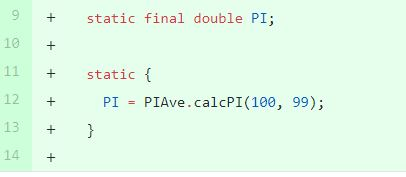
\includegraphics{Image/Singleton.JPG}
    \end{center}
    
    \item Avoid Hard Coding Value, create a constants file and register all constants value in that file.  
    \begin{center}
    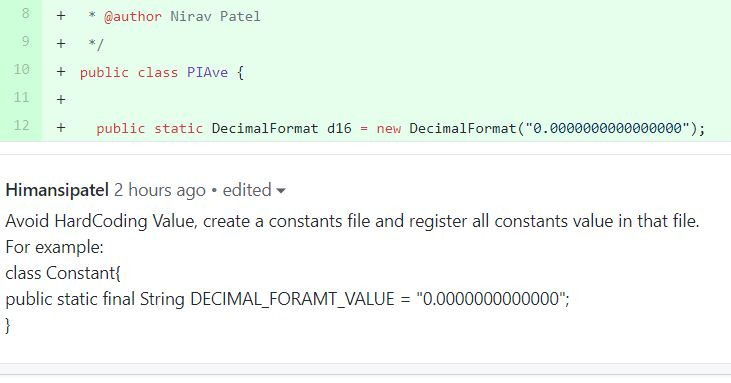
\includegraphics[width=14cm, height=8cm]{Image/hardcodedvalue.JPG}
    \end{center}
   
    \item Proper naming convention to follow
    \begin{center}
    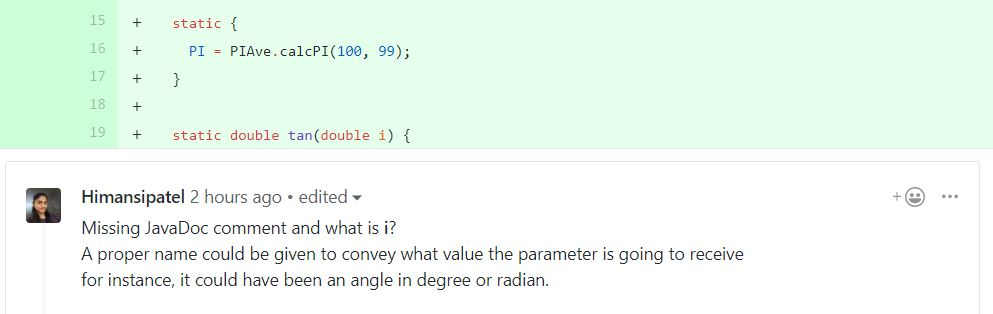
\includegraphics[width=16cm, height=8cm]{Image/commentmissing.JPG}
    \end{center}
    
    \item  For the validator.java, it validates whether the input and output is in valid range or not, it checks for the different condition and prints the same message, which can be combined in single if condition by making use of logical OR condition.
    \begin{center}
    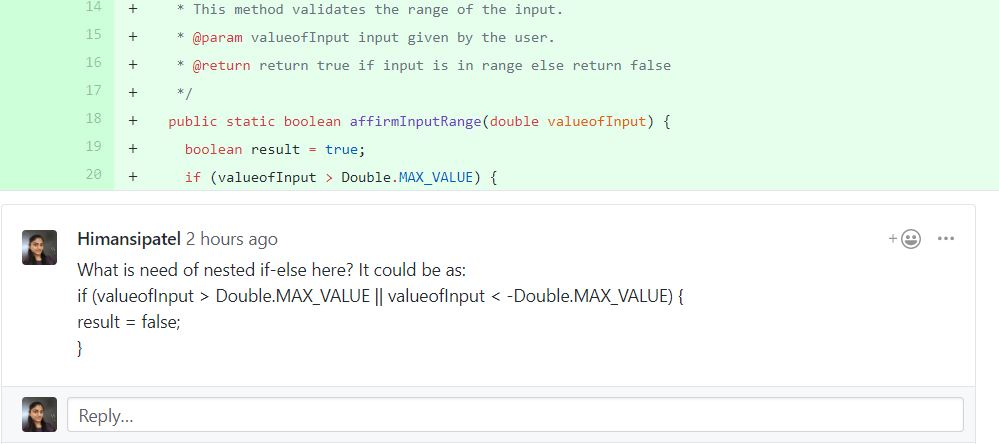
\includegraphics[width=16cm, height=8cm]{Image/reduceif.JPG}
    \end{center}
    
\end{enumerate}
\newpage

\section{Problem 7}
\subsection{Test Cases Analysis for Function $f(x)=sinh(x)$}
Functional testing is a phase in software development which involves testing and verifying the functional requirements of system. It is generally accomplished in various forms and levels like unit testing at developers end, integration testing and system testing by QA teams. \\
Its is a quality assurance (QA) process and is generally considered to be a type of black-box testing that bases its test cases on the specifications of the software component under test. Functions are tested by feeding them input and examining the output.\cite{testing}\\
We have specifically used : \\
1. Black-box testing approach ignoring the internal design of the system and just ensuring if the results align well with the intended behaviour.\\
2. Some boundary value testing to handle edge cases that are not explicitly covered in the functional requirements.
\\\\
Functional testing primarily involves the given steps
\begin{enumerate}
    \item Identifying the core functionalities that the system is expected to perform
    \item Creating/Mocking input data sets for the test cases, in alignment with system's functional requirements.
    \item Determining outputs for the prepared input data sets.
    \item Executing the test suit and thereon comparing actual and expected outputs.
    \item Checking if the application behaves as intended and respect the functional specifications.
\end{enumerate}
The summary tables for the test cases are described below which compares the actual output with the expected output based on input and give status.
\subsubsection{Test Case Method : testInitCalculationInvalidInput()}
This unit test is tested on improper inputs like string and combinations of special characters and it return the expected response.
\subsubsection{Test Case Method : testInitCalculationInvalidUpperBoundInput()}
This test task was to identify the upper bound value and if it exceeds the threshold value this unit function is returning the expected response.
\subsubsection{Test Case Method : testInitCalculationValidInput() }
This test is expected to receive the proper value as input and return the result, but this unit function works for some real integers.
\begin{center}
\begin{tabular}{ |c|c|c|c| } 
\hline
\textbf{Input} & \textbf{Expected Result} & \textbf{Actual Result} & \textbf{Status} \\
\hline
9 & 4051.54190208 & 3991.013168667828000 & Failed \\ 
\hline
1 & 1.1752011936438 & 1.1752011936438 & Passed \\ 
\hline
\end{tabular}
\end{center}
\subsubsection{Test Case Method : testEPowerXFinite()}
This test case is expected to calculate Euler value with respective finite value of x and it is returning the expected value of $e^x$.
\subsubsection{Test Case Method : testCalculateSinh() }
This test is use for calculating value of sinh which accepts 2 parameters $e^x$ and $e^{-x}$ and returns the expected value for some real number of sinh function.
\begin{center}
\begin{tabular}{ |c|c|c|c|c| } 
\hline
\textbf{Input1} & \textbf{Input2} & \textbf{Expected Result} & \textbf{Actual Result} & \textbf{Status} \\
\hline
9 & -9 & 4051.54190208 & 3991.013168667828000 & Failed \\ 
\hline
1 & -1 & 1.1752011936438 & 1.1752011936438 & Passed \\ 
\hline
\end{tabular}
\end{center}
\subsubsection{Test Case Method : testSignificantDecimalPoints() }
This test just verifies that input given by user, contains max 15 decimal significant points which will then use as processedInput.
\begin{center}
\begin{tabular}{ |c|c|c|c| } 
\hline
\textbf{Input} & \textbf{Expected Result} & \textbf{Actual Result} & \textbf{Status} \\
\hline
0.000000000000000000000 & 0.000000000000000 & 0.000000000000000 & Passed \\ 
\hline
0.12 & 0.12 & 0.12 & Passed \\ 
\hline
\end{tabular}
\end{center}
\subsubsection{Test Case Method : testValidateInputRangeInvalidInput() }
This test is working correctly for detecting that the input value should lie within the given interval.
\begin{center}
\begin{tabular}{ |c|c|c|c| } 
\hline
\textbf{Input} & \textbf{Expected Result} & \textbf{Actual Result} & \textbf{Status} \\
\hline
2*Double.MAX\_VALUE & false & false & Passed \\ 
\hline
\end{tabular}
\end{center}
\subsubsection{Test Case Method : testValidateOutputRange }
This test is working properly for the cases where output reaches to too large value which cannot be stored or not in range.
\begin{center}
\begin{tabular}{ |c|c|c|c| } 
\hline
\textbf{Input} & \textbf{Expected Result} & \textbf{Actual Result} & \textbf{Status} \\
\hline
2*Double.NEGATIVE\_INFINITY & false & false & Passed \\ 
\hline
2*Double.POSITIVE\_INFINITY & false & false & Passed \\ 
\hline
9 & true & true & Passed\\
\hline
\end{tabular}
\end{center}
\subsubsection{Results}
\begin{figure}[h!]
    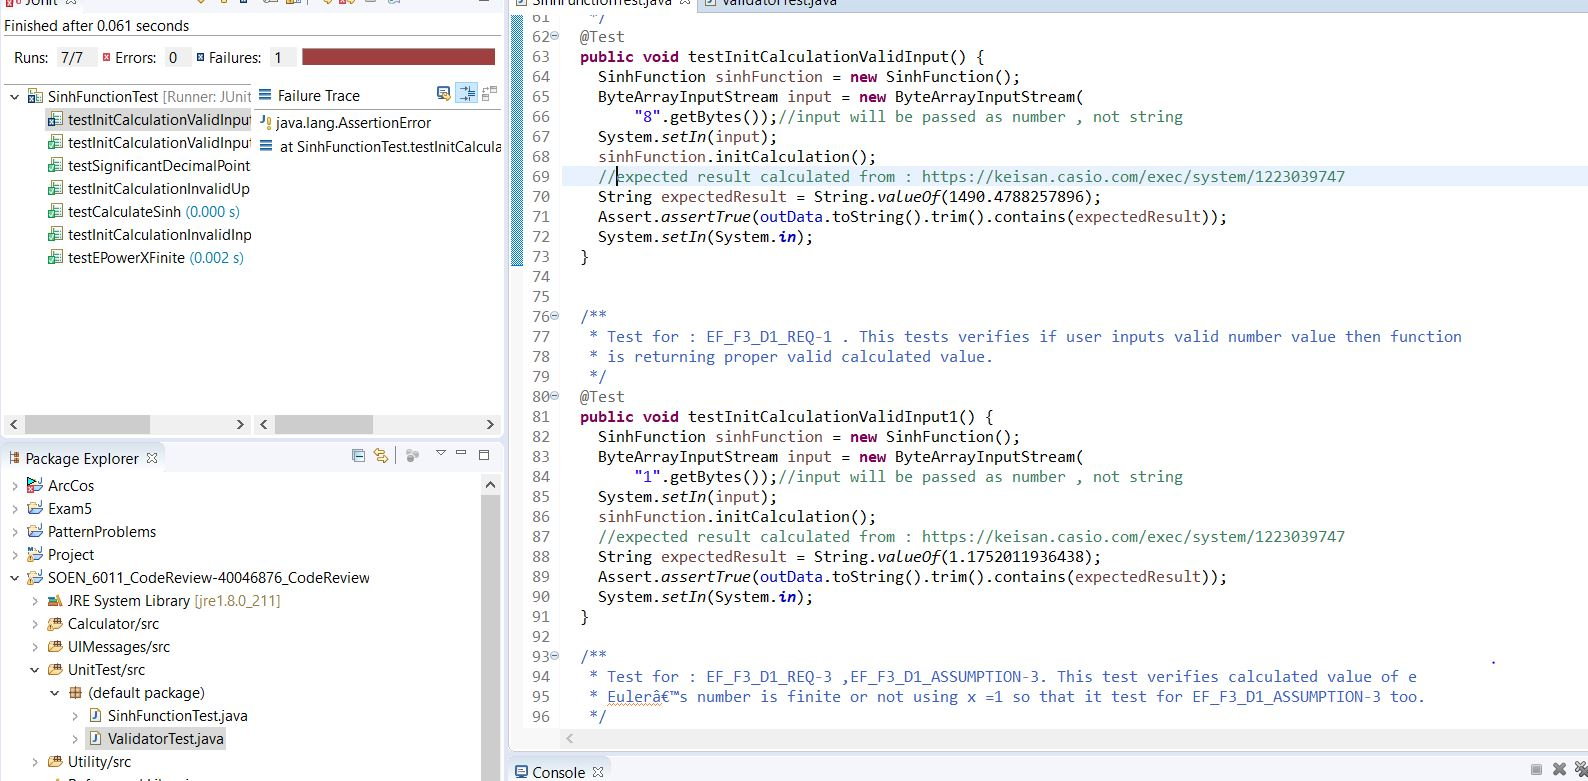
\includegraphics[width=16cm, height=10cm]{Image/testcasesinh.JPG}
    \caption{Execution of test cases for SinhFunctionTest.java}
\end{figure}
\begin{figure}[h!]
    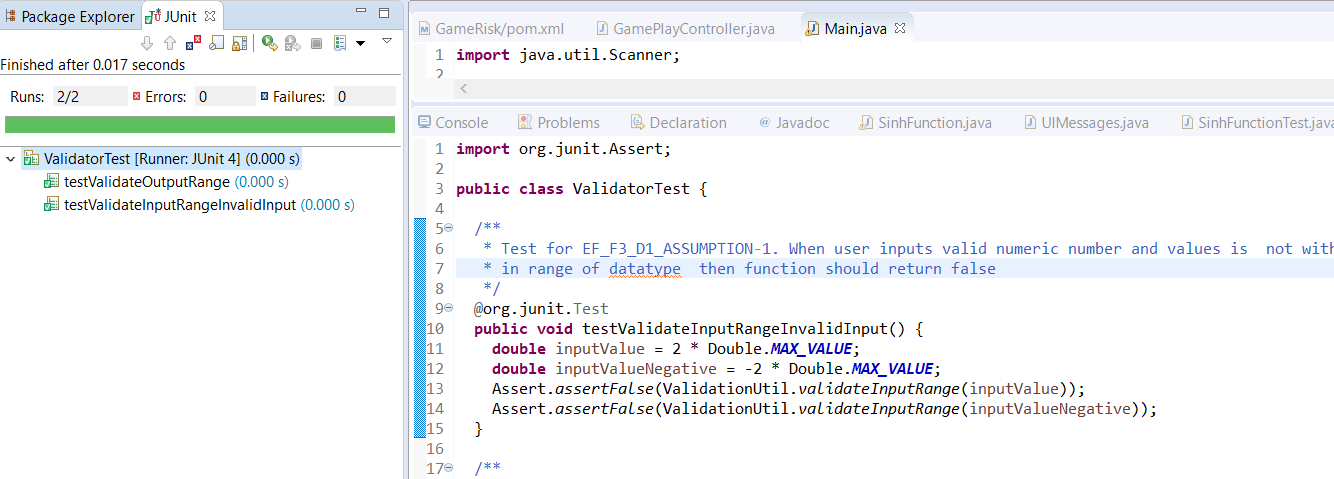
\includegraphics[width=16cm, height=10cm]{Image/testReview2.png}
    \caption{Execution of test cases for ValidatorTest.java}
\end{figure}
\clearpage
\newpage
\section{Version Control System}
For code Review : -\\
\url{https://github.com/niravjdn/SOEN-6011-Project-Team-H-Nirav/pull/2/files}
For Test Case Analysis : - \\
\url{https://github.com/prashantp995/SOEN_6011_CodeReview}

\begin{thebibliography}{9}
\bibitem{testing}
\url{https://www.softwaretestinghelp.com/guide-to-functional-testing/}
\bibitem{pmd}
\url{https://marketplace.eclipse.org/content/pmd-eclipse-plugin}
\end{thebibliography}


\end{document}